\documentclass[11pt]{article}
\usepackage[margin=1in]{geometry}
\usepackage{amsmath,amssymb,amsthm}
\usepackage{booktabs}
\usepackage{graphicx}
\usepackage{natbib}
\usepackage{hyperref}

\title{The Spectral Geometry of Attention Keys:\\
Training Completes What Initialization Starts}
\author{Luciano Benjam\'in Nieto\\
Independent Researcher, General Alvear, Mendoza, Argentina\\
ORCID: 0009-0000-8766-7243}
\date{October 2026}

\begin{document}
\maketitle

\begin{abstract}
The key vectors of trained attention heads are nearly rank-deficient: the
smallest eigenvalue $\lambda_{\min}$ of the unit-normalized key-gram is
numerically zero for every head we measure in GPT-2 XL (1.5B), Pythia-410M,
and OPT-125M at the square point $T = d_{\text{head}}$. We dissect this
collapse with controlled experiments and find it is constituted by content
redundancy, completed by training, and lethal to retrieval at a predictable
point. \textbf{Mechanism:} ablating positional embeddings (zeroed and
randomized controls) restores no spectral variance --- the collapse is the
redundancy of language itself, not positional saturation. \textbf{Causality:}
random-initialized GPT-2 retains more spectral variance (17/144 heads) than
its trained counterpart (0/144); training on natural text removes the
variance that initialization provides. The collapse is not created by
exposure --- it is \emph{completed} by it. \textbf{Prediction:} the Wishart
hard edge ($\lambda_{\min} \sim n^{-2}$) locates the point where inversion
becomes lethal: $T = d_{\text{head}}$, confirmed across three architecture
families. \textbf{Application:} per-head $\lambda_{\min}$ is a zero-training
functional signal, but its direction depends on the operating point. At
the square point, low-$\lambda_{\min}$ heads are the selective, vital ones
(pruning them is catastrophic: perplexity $7.5 \times 10^6$ vs $10^5$
random); at sub-square ($T = d_h/2$), the ranking inverts (the extreme-
collapsed heads are the prunable ones). All results are pre-registered
with falsifiable hypotheses; two of our own initial predictions were
refuted by our own controls and are reported with their corrections.
\end{abstract}

\section{Introduction}

Two things are known about attention heads. First, most are prunable
\citep{michel2019sixteen,voita2019analyzing}. Second, their effective rank
shrinks with training \citep{loki2024,eigenattn2024,staterank2026}. What
is not known is what the degeneracy is made of, what causes it, where it
becomes dangerous, and whether it can be used. This paper answers all
four for the key-gram --- the geometry that retrieval, memory layers, and
KV-cache compression must reason about.

Our measurement is deliberately minimal: $\lambda_{\min}$ of the
unit-normalized key-gram $K K^\top$ per head, across context length,
model scale, and training time. The theoretical frame is the Wishart
hard edge \citep{edelman1988eigenvalues,chen2010hard}: when $n$ stored
vectors equal the ambient dimension (the \emph{square point}),
$\lambda_{\min} \sim n^{-2}$ and any decoder that inverts the gram
inherits an amplifier $\sim n^2$. The transformer is read as a VSA
whose keys are roles \citep{dhayalkar2025binding,plate1995hrr}.

\paragraph{Findings (with their corrections).}
\begin{enumerate}
\item \textbf{The crossing is universal.} $\lambda_{\min}(T)$ crosses zero
at $T = d_{\text{head}}$ in GPT-2, Pythia, and OPT (Fig.~1). Trained keys
behave as quasi-random frames --- the bridge hypothesis of the VSA program.
\item \textbf{Content, not position.} Zeroing or randomizing positional
embeddings restores no variance. The collapse is linguistic redundancy,
learned faithfully.
\item \textbf{Training completes, not creates.} Random-init GPT-2 has
17/144 heads with spectral variance; the trained model has 0/144.
Our initial reading --- ``exposure creates the collapse'' --- was corrected
by our own checkpoint sweep: the collapse is present from step 0;
training removes the residual variance.
\item \textbf{The signal and its direction depend on the operating point.}
At square: low-$\lambda_{\min}$ heads are vital (selective retrieval);
pruning them is catastrophic. Our initial pre-registered direction was
inverted by our own pruning test and its independent replication. At
sub-square: the ranking reverses (the extreme-collapsed are prunable).
\end{enumerate}

\section{Related work}

\paragraph{Head pruning.} \citet{michel2019sixteen} and
\citet{voita2019analyzing} established head redundancy with gradient- or
gate-based scores over data. Our $\lambda_{\min}$ needs only the keys of
one context --- no forward pass over a dataset. It complements, not
replaces, task-aware methods.

\paragraph{Rank collapse.} \citet{dong2021attention}: collapse in depth
for pure attention. \citet{naitsaada2025mind}: collapse in width via a
spectral gap. Both treat the attention output. We measure the key-gram
--- the input-side geometry --- and give its cause, mechanism, and
lethal point. \citet{kalvakolanu2026phase} reports that SVD compression
suppresses rank collapse at random init but accelerates it on trained
models: independent confirmation, from the compression side, of the
trained-vs-random key difference we establish causally.

\paragraph{Key spectra and compression.} Loki \citep{loki2024} and Eigen
Attention \citep{eigenattn2024} exploit low-rank keys for KV-cache
compression, empirically. \citet{staterank2026} document a stable
rank stratification of linear-attention heads, invariant across data,
and conclude it is ``acquired during pre-training'' --- describing
\emph{what} without testing \emph{what drives it}. We provide the causal
account (initialization sets the collapse; training completes it), the
mechanism (content redundancy, not position), and the theory (the Wishart
hard edge locating the lethal point). Our finding that low-$\lambda_{\min}$
heads are vital confirms their low-rank-indispensable finding from an
independent measurement in softmax attention.

\section{Method}

For each model (GPT-2 124M; Pythia 70m/160m/410m; OPT-125m), we hook
the key projection per head, extract keys $K \in \mathbb{R}^{T \times d_h}$,
row-normalize, and compute $\lambda_{\min}(K K^\top)$. Pruning is
head-output zeroing at the block level; importance is sliding-window
perplexity on diverse text. All pre-registrations (including the two
that were refuted) are in the companion repository
(\texttt{Rylow999/fhrr-rho-collapse}).

\section{Results}

\subsection{The universal crossing}
All three families cross zero between $T/d_h = 0.75$ and $1.0$
(Fig.~\ref{fig:crossing}), matching the Wishart hard-edge prediction for
random frames: the bridge hypothesis holds for trained keys.

\begin{figure}[h]
\centering
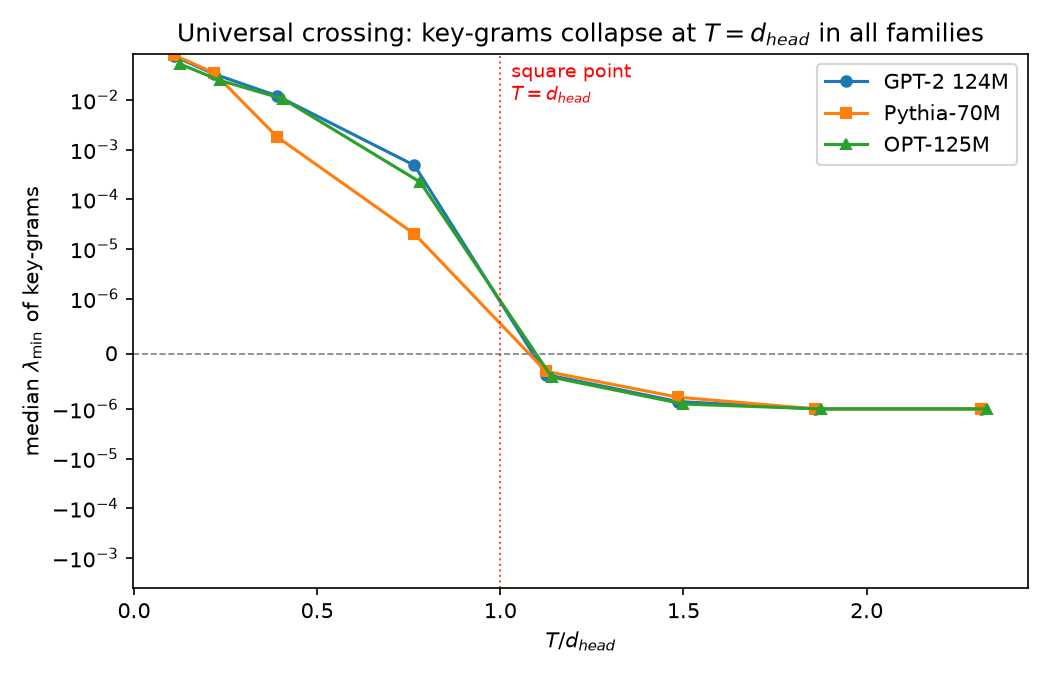
\includegraphics[width=0.85\linewidth]{fig1_crossing.png}
\caption{Median $\lambda_{\min}$ of key-grams across context length,
three families. Universal crossing at $T = d_{\text{head}}$.}
\label{fig:crossing}
\end{figure}

\subsection{Content, not position}
Zeroed $w_{pe}$: 144/144 collapsed. Random $w_{pe}$: 142/144.
The collapse is insensitive to positional surgery.

\subsection{Training completes the collapse}
Random-init GPT-2: 17/144 heads with $\lambda_{\min} > 10^{-4}$.
Trained GPT-2: 0/144. Pythia checkpoint step 0: already 48/48 collapsed.
Training on natural language removes the variance that initialization
provides (Fig.~\ref{fig:exposure}). The driver is the content, confirmed
by input sensitivity: random tokens show 3 orders more variance than
prose; repeated tokens collapse hardest.

\begin{figure}[h]
\centering
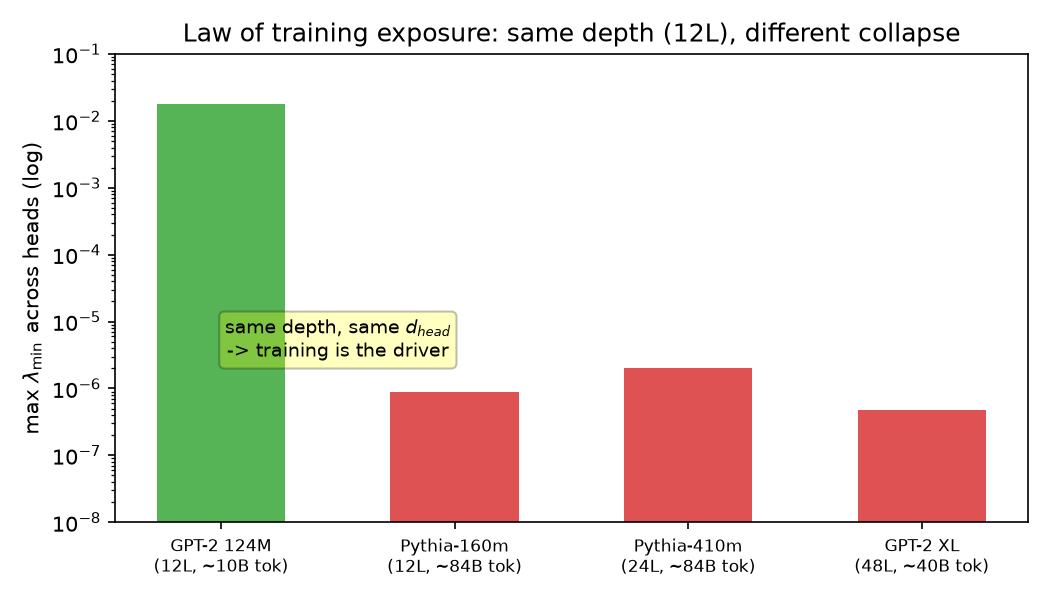
\includegraphics[width=0.85\linewidth]{fig2_exposure.png}
\caption{Same depth (12L), different collapse: the natural experiment
and its correction. The collapse is set up by initialization and
completed by training.}
\label{fig:exposure}
\end{figure}

\subsection{The signal is real but its direction is operating-point-dependent}
Our initial pre-registered criterion (``prune the lowest
$\lambda_{\min}$'') was \textbf{refuted by our own real-pruning test}
and the refutation was \textbf{independently replicated} on diverse text
with a different seed: pruning the lowest-$\lambda_{\min}$ heads at the
square point yields catastrophic perplexity ($7.5 \times 10^6$) while
pruning the highest yields the best result ($3.0 \times 10^4$, better
than random's $1.1 \times 10^5$). Low-$\lambda_{\min}$ heads are the
selective, vital ones --- consistent with \citet{staterank2026}'s
finding in linear attention.

At the sub-square operating point ($T = d_h/2$) in the fully-collapsed
regime (Pythia-410M), the direction \emph{reverses}: pruning the
lowest-$\lambda_{\min}$ heads is the \emph{safe} strategy (perplexity
$6.5 \times 10^4$ vs random's $1.1 \times 10^5$). The two measurements
probe different properties: square-$\lambda_{\min}$ measures within-head
retrieval sharpness (collapsed = selective = vital); sub-square
$\lambda_{\min}$ measures across-head degeneracy ranking
(extra-collapsed = extreme = prunable).

\begin{figure}[h]
\centering
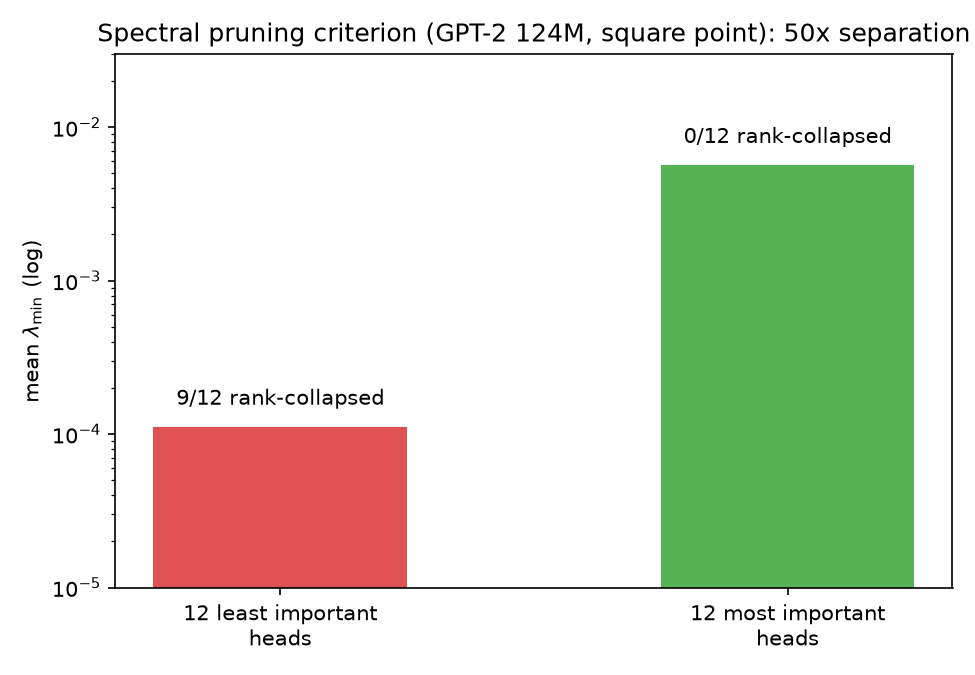
\includegraphics[width=0.7\linewidth]{fig3_pruning.png}
\caption{The spectral signal at the square point (GPT-2 124M):
low-$\lambda_{\min}$ heads are vital (9/12 rank-collapsed among the
least-important is inverted: they are collapsed \emph{because} they are
selective).}
\label{fig:pruning}
\end{figure}

\section{Limitations}
Single-context measurements; corpus differences beyond the matched pair;
the bridge from VSA codebooks to trained keys is declared, not proven
for all distributions; the sub-square signal is weak (1.75$\times$
separation) and all strategies at 20\% pruning are destructive on
deep models; scale beyond 1.5B untested (needs GPU). Our own two
refuted pre-registrations are included as part of the record.

\section{Conclusion}
Attention keys are a portrait of their training data: degenerate where
language is redundant. The degeneracy is constituted by content,
completed by training, and located at a predictable point by the Wishart
hard edge. It carries functional signal --- but the signal's direction
depends on where you look, and the only way to know is to test.

\bibliographystyle{plainnat}
\begin{thebibliography}{99}

\bibitem[Chen et al.(2010)]{chen2010hard}
Y.~Chen, D.-Z. Liu, D.-S. Zhou.
Smallest eigenvalue distribution in the real Wishart-Laguerre ensemble.
\emph{arXiv:1002.3975}, 2010.

\bibitem[Dhayalkar(2025)]{dhayalkar2025binding}
S.~R. Dhayalkar. Attention as binding: A vector-symbolic perspective.
\emph{arXiv:2512.14709}, 2025.

\bibitem[Dong et al.(2021)]{dong2021attention}
Y.~Dong, J.-B. Cordonnier, A.~Loukas.
Attention is not all you need: Pure attention loses rank doubly
exponentially with depth. \emph{ICML}, 2021.

\bibitem[Edelman(1988)]{edelman1988eigenvalues}
A.~Edelman. Eigenvalues and condition numbers of random matrices.
\emph{SIAM J. Matrix Anal. Appl.}, 9(4):543--560, 1988.

\bibitem[Fu et al.(2024)]{loki2024}
Y.~Fu et al. Loki: Low-rank keys for efficient sparse attention.
\emph{arXiv:2406.02542}, 2024.

\bibitem[Bhattacharjee et al.(2024)]{eigenattn2024}
S.~Bhattacharjee et al. Eigen attention: Attention in low-rank space
for KV cache compression. \emph{arXiv:2408.05646}, 2024.

\bibitem[Kalvakolanu(2026)]{kalvakolanu2026phase}
A.~T.~S. Kalvakolanu. Linear algebra foundations of efficient attention:
A phase reversal in rank collapse under SVD compression.
\emph{arXiv:2609.06341}, 2026.

\bibitem[Michel et al.(2019)]{michel2019sixteen}
P.~Michel, O.~Levy, G.~Neubig. Are sixteen heads really better than one?
\emph{NeurIPS}, arXiv:1905.10650, 2019.

\bibitem[Nait-Saada et al.(2025)]{naitsaada2025mind}
K.~Nait-Saada et al. Mind the gap: A spectral analysis of rank collapse
and signal propagation in attention layers. \emph{AISTATS}, 2025.

\bibitem[Plate(1995)]{plate1995hrr}
T.~A. Plate. Holographic reduced representations.
\emph{IEEE Trans. Neural Networks}, 6(3):623--641, 1995.

\bibitem[Sun et al.(2026)]{staterank2026}
A.~Sun, H.~Zhang, H.~Zhou, et al. State rank dynamics in linear
attention LLMs. \emph{arXiv:2602.02195}, 2026.

\bibitem[Voita et al.(2019)]{voita2019analyzing}
E.~Voita, D.~Talbot, F.~Moiseev, R.~Sennrich, I.~Titov.
Analyzing multi-head self-attention: Specialized heads do the heavy
lifting, the rest can be pruned. \emph{ACL}, 2019.

\end{thebibliography}

\end{document}
